\begin{figure}
    \centering
    \includegraphics[width=12cm]{../figures/blip_bbh_runs_two_panel_comparison.pdf}
    \caption{Glitch panel comparison}
    \label{fig:qscan_null}
\end{figure}

\begin{figure}
    \centering
    \includegraphics[width=10cm]{../figures/et2l_delta_glitch_overlap_glitch_master.pdf}
    \caption{Glitch overlap}
    \label{fig:glitch_overlap}
\end{figure}

\begin{figure}
    \centering
    \includegraphics[width=10cm]{../figures/newsnr_mismatch_comparison.pdf}
    \caption{Mismatch}
    \label{fig:mismatch}
\end{figure}

\begin{figure}
    \centering
    \includegraphics[width=16cm]{../figures/newsnr_fig_4.pdf}
    \caption{Mass Distance Sky}
    \label{fig:delta_zero}
\end{figure}

\begin{figure}
    \centering
    \includegraphics[width=10cm]{../figures/newsnr_rank_10_single_block_percentile_parameters_short.pdf}
    \caption{Confidence interval}
    \label{fig:trend_delta}
\end{figure}


\begin{figure}
    \centering
    \includegraphics[width=16cm]{../figures/assemble_nijntje.pdf}
    \caption{The workflow of Nijntje algorithm. \textit{Step 1}:Lorem. \textit{Step 2}: Ipsum. \textit{Step 3}: Lorem. \textit{Step 4}:Ipsum.}
    \label{fig:nijntje_chart}
\end{figure}

